\section{Neural Networks}\label{sec:neural-networks}

\begin{frame}{Perceptron}
    \begin{columns}
        \column{\moit} \textbf{Perceptron}: Model inspired by the functioning of neurons in the human brain, provide a mathematical model that enabled machines to learn from data and make predictions~\cite{rosenblatt1958perceptron}.
        \column{\moit} \begin{figure}[ht]
                                \centering
                                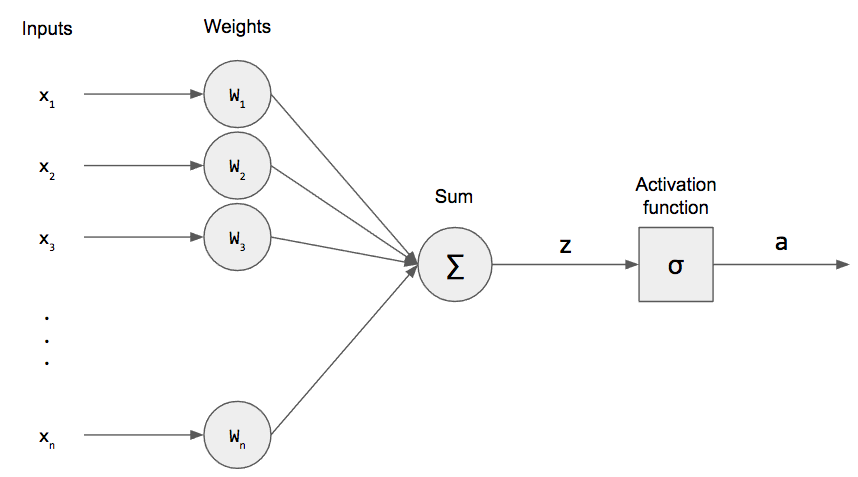
\includegraphics[width=\textwidth]{imgs/Single-Perceptron.png}
                                \caption{Illustration of an LTU, which are the building blocks of neural networks}
                                \label{fig:perceptron}
                            \end{figure}
    \end{columns}
\end{frame}


\begin{frame}{Neural networks}
    \begin{columns}
        \column{\moit} Also known as \emph{multi-layer} perceptron. 
                    \begin{enumerate}
                        \item Input layer for the data $\Vec{x}$
                        \item Hidden layers
                        \item Output layer for the network's prediction $\hat{f}_{\Vec{x}}$
                    \end{enumerate}{}
                     Output of layer $l$ can be expressed as:
                        \begin{equation*}
                            \label{eq:output-any-layer}
                            \Vec{a}^{(l)} = \sigma^{(l)}\left(\mathbf{W}^{(l)} \cdot \Vec{a}^{(l-1)} + \Vec{b}^{(l)}\right)
                        \end{equation*}
        \column{\moit} \begin{figure}[ht]
                            \centering
                            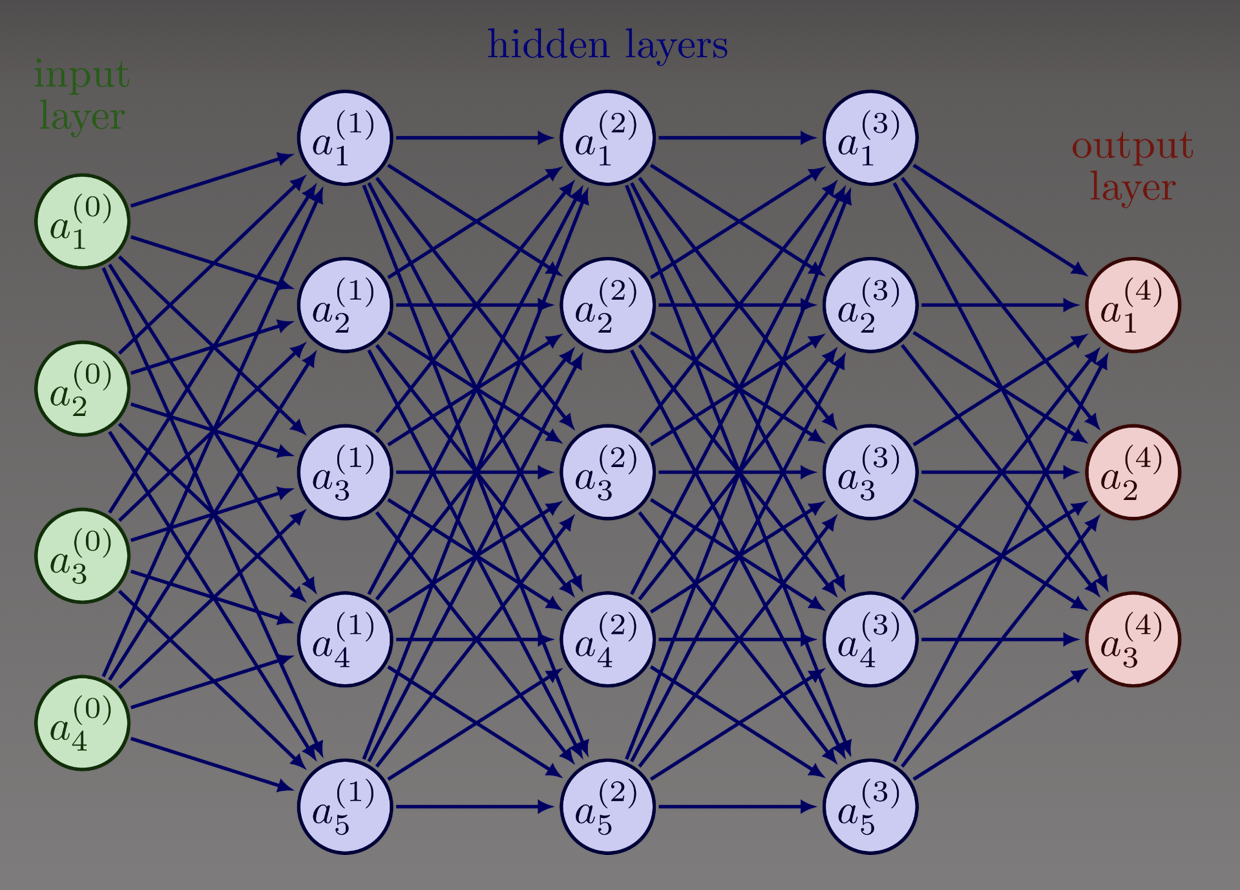
\includegraphics[width=\textwidth]{imgs/Architecture-perceptron-multi-couches-2.png}
                            \caption{Structure of a neural network with three hidden layers.}
                            \label{fig:mlp}
                        \end{figure}
                       
    \end{columns}
\end{frame}

\begin{frame}{Neural Networks}
    A neural network is a mathematical function. Can be described as a series of nested non-linear functions:

\begin{align}
f &\text{: } \mathbb{R}^n \to \mathbb{R}^m\nonumber\\
f &= g \circ f_L \circ f_{L-1} \dots f_2 \circ f_1 (x) \text{ with, }
\end{align}

\begin{align}
f_l &\text{: } \mathbb{R}^{n_l} \to \mathbb{R}^{n_{l-1}}\nonumber\\
f_l&(x) = \sigma^{(l)}(\mathbf{W}^{(l)} \cdot \Vec{x} + b^{(l)})
\end{align}

$n$ : dimension of the input $\Vec{x}$, $m$ : dimension of the output $\Vec{y}$, $g$: \emph{output function}
\end{frame}


\begin{frame}{Loss Function}
    Quantification of the error produced by the network via a \emph{loss function}. Commonly used Mean Squared Error (MSE):
    \begin{equation*}
        \label{eq:def-loss-function}
        \mathcal{L}(\theta) = \frac{1}{2n} \sum_{i=1}^n \left[\hat{y}_{\theta}^{(i)} - y^{(i)}\right]^2
    \end{equation*}
    $\theta$: set of parameters (weights and biases), $\hat{y} = \hat{f}(\Vec{x})$: value predicted, $y=f(\Vec{x})$: \emph{real} value.
\end{frame}


\begin{frame}{Gradient Descent}
    Method to udpdate network's parameters: \emph{Gradient descent}~\cite{cauchymethode}
    \begin{columns}
        \column{\moit} Parameters $\theta$  at step $n+1$ are updated:
            \begin{equation*}
                    \label{eq:gradient-descent}
                    \Vec{\theta}_{n+1} = \Vec{\theta}_n - \eta \nabla \mathcal{L}(\Vec{\theta}_n)
            \end{equation*}
            $\eta \in \mathbb{R}^+$ is called \emph{learning rate}.
        \column{\moit} 
        \begin{figure}
            \centering
            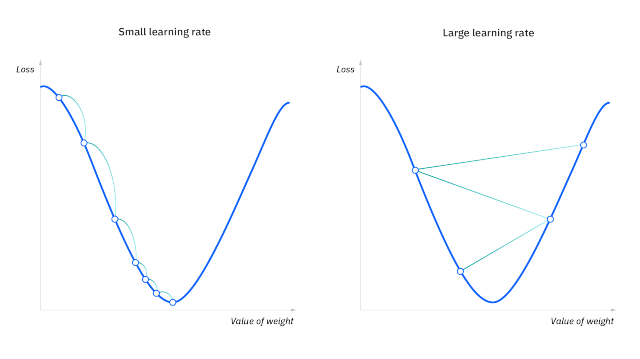
\includegraphics[width=\textwidth]{imgs/desc-grad.png}
            \caption{Influence of the learning rate on the convergence of the loss.}
        \end{figure}
    \end{columns}
\end{frame}


%\begin{frame}{Back-propagation}



%\only<1>{Algorithm that enables the computation of the gradient of the error, thereby permitting the adjustment of network parameters according to~\eqref{eq:gradient-descent}.
%\begin{figure}
%    \centering
%    \begin{tikzpicture}

%        \node[draw,rectangle,minimum height=2cm,minimum width=3cm,align=center] (layer) at (0,0) {Layer $l$};
        
%         \draw[<-] ([yshift=0.5cm]layer.west) -- ++(-3,0) node[midway,above] {$X^{(l)}=a^{(l-1)}$};
%         \draw[->] ([yshift=-0.5cm]layer.west) -- ++(-3,0) node[midway,below] {$\frac{\partial E}{\partial X^{(l)}}$};
        
%         \draw[->] ([yshift=0.5cm]layer.east) -- ++(3,0) node[midway,above] {$a^{(l)}=X^{(l+1)}$};
%         \draw[<-] ([yshift=-0.5cm]layer.east) -- ++(3,0) node[midway,below] {$\frac{\partial E}{\partial a^{(l)}} $};
%     \end{tikzpicture}
%     \caption{Hidden layer $l$ of a neural network.}
%     \label{fig:illustration-layer-l}
% \end{figure}}

% \only<2>{The  algorithm can be summarized in three main steps:
% \begin{enumerate}
%     \item Compute the forward pass for each input-output pair by proceeding from layer 1, the input layer, to layer $L$, the output layer.
%     \item Compute the backpward phase for each input-output pair by proceeding from layer $L$, the output layer, to layer 1, the input layer. 
%     %\begin{enumerate}
%     %   \item Evaluate the error term for the final layer.
%     %   \item Backpropagate the error terms for the hidden layers, starting from the last hidden layer $l=L-1$.
%     %   \item Evaluate the partial derivatives of the error with respect to $w_{ik}^{(l)}$ 
%     %\end{enumerate}
%     \item Update the parameters according to the gadient descent algorithm.
% \end{enumerate}

% One full cycle of this algorithm is called an \emph{epoch}.}
% \end{frame}

\begin{frame}{Important Properties}

    \begin{itemize}
        \item \textbf{Universal Approximation Theorem}: asserts that a neural network with a single hidden layer can approximate any continuous function on compact subsets of $\mathbb{R}^n$, provided that the hidden layer's activation function is non-constant, bounded, and continuous.
        \item \textbf{Automatic Differentiation}: Efficient way of computing derivatives with no approximation error.
    \end{itemize}
    
\end{frame}
